\documentclass{article}
\usepackage[utf8]{inputenc}
\usepackage{graphicx}
\usepackage{amssymb}
\usepackage{amsmath, nicefrac}
\usepackage{amsthm}
\usepackage{microtype}
\usepackage{bm}
\usepackage{bbm}
\usepackage{algorithm, algorithmicx, algpseudocode}
\usepackage{/home/amice/Desktop/Own}

\usepackage{geometry}
\geometry{margin=1in}

\newcommand{\mat}[1]{\bm{#1}}
\newcommand{\bmat}[1]{\begin{bmatrix} #1 \end{bmatrix}}

\DeclareMathOperator{\sgn}{sgn}
\let\diag\relax
\DeclareMathOperator{\diag}{diag}

\newcommand{\inputtikz}[2]{%  
     \scalebox{#1}{\input{#2}}  
}

\title{ESE 650, Spring 2019 Assignment 3}
\date{Due March 15, 2019}
\author{Alexandre Amice}

\begin{document}

\maketitle

\section{Part 1 (30 Points)}

 
\begin{enumerate} 
  % Problem
  \item   Suppose that the pose of a moving robot with respect to the world frame is given by the following function of time $t$:
  \[
  T(t) = \begin{bmatrix}
    \cos\frac{t\pi}{3}  & 0 & -\sin\frac{t\pi}{3} & t\\
    0  &  1 &  0 &0\\
    \sin\frac{t\pi}{3} &  0 & \cos\frac{t\pi}{3} & 2t\\
    0 & 0 & 0 & 1
  \end{bmatrix} \in SE(3)
  \]
  Note that 
  \begin{align*}
   T(1) = \begin{bmatrix}
    \cos\frac{\pi}{3}  & 0 & -\sin\frac{\pi}{3} & 1\\
    0  &  1 &  0 &0\\
    \sin\frac{\pi}{3} &  0 & \cos\frac{\pi}{3} & 2\\
    0 & 0 & 0 & 1
  \end{bmatrix} = \begin{bmatrix}
    \frac{1}{2}  & 0 & -\frac{\sqrt{3}}{2} & 1\\
    0  &  1 &  0 &0\\
    \frac{\sqrt{3}}{2} &  0 & \frac{1}{2} & 2\\
    0 & 0 & 0 & 1
  \end{bmatrix}
  \end{align*}
  Also we will follow the convention
  \begin{align*}
   T(t) = \begin{bmatrix}
           R(t) & s(t) \\
           0 & 1
          \end{bmatrix}
  \end{align*}


    \begin{enumerate}
      \item \textbf{Find the axis-angle representations of the robot orientation at time $t=1$}. \\\\
      The rotation component of the matrix $T(1)$ is 
      \begin{align*}
      \begin{bmatrix}
       \frac{1}{2}  & 0 & -\frac{\sqrt{3}}{2} \\
    0  &  1 &  0\\
    \frac{\sqrt{3}}{2} &  0 & \frac{1}{2} 
      \end{bmatrix}
      \end{align*}
      From the Rodrigues formula we have
      \begin{align*}
       \tr(R) = 1 + 2 \cos(\theta) &= \frac{1}{2} + \frac{1}{2} + 1
       \\
       \Rightarrow 2 \cos(\theta) &= 1
       \\
       \theta &= \arccos\left(\frac{1}{2}\right)
       \\
       \theta &= \frac{\pi}{3}
      \end{align*}
      and
      \begin{align*}
       R-R^T &= 2\sin(\theta) \hat \omega
       \\
       \Rightarrow \begin{bmatrix}
                0 & 0 & -\sqrt{3} \\
                0 & 0& 0 \\
                \sqrt{3} & 0 & 0
               \end{bmatrix} &=  2 \sin\left(\frac{\pi}{3}\right) \hat \omega
      \\
      \begin{bmatrix}
                0 & 0 & -\sqrt{3} \\
                0 & 0& 0 \\
                \sqrt{3} & 0 & 0
               \end{bmatrix} &=  \sqrt{3} * \hat \omega
               \\
               \hat \omega &= \begin{bmatrix}
                0 & 0 & -1 \\
                0 & 0& 0 \\
                1 & 0 & 0
               \end{bmatrix}
               \\
               \Rightarrow \omega &= \begin{bmatrix}
                                      0 \\ -1 \\ 0
                                     \end{bmatrix}
      \end{align*}



      \item \textbf{Find the quaternion representations of the robot orientation at time $t=1$ and of the inverse of this orientation.} \\\\
      Using the angle and axis from part (a) we have that
      \begin{align*}
       q &= \left( \cos\left(\frac{\theta}{2}\right), \sin\left(\frac{\theta}{2}\right) \omega \right)
       \\
       &= \left( \cos\left(\frac{\pi}{6}\right), \sin\left(\frac{\pi}{6}\right) \begin{bmatrix}
       0 & -1 & 0
       \end{bmatrix}^T\right)
       \\
      &= \left( \frac{\sqrt{3}}{2}, 0 , -\frac{1}{2}, 0 \right)
      \end{align*}
      The inverse of the orietation is given by the conjugate of the quaternion which is simply
      \begin{align*}
       q^* = \left( \frac{\sqrt{3}}{2}, 0 , \frac{1}{2}, 0 \right)
      \end{align*}


      \item \textbf{Compute the linear and the angular velocity with respect to the world frame at time $t = 1$.} \\\\
   
      Note that we have 
      \begin{align*}
       R(t)R(t)^T &= I \\
       R'(t)R(t)^T +R(t)R'(t)^T &= 0
       \\
       \Rightarrow
       R'(t) &= -R(t)R'(t)^TR(t)
       \\
       \Rightarrow R'(t) &= R'(t)R^T(t) R(t) = S(\omega(t)) R(t)
      \end{align*}
      Where $S$ is skew symmetric because it is the rigid rotation of a skew symmetric matrix. We prove that $S(\omega(t))$ is the matrix representing the angular velocity vector by consider two points $p^0, p^1$ attached to the rigid body, and the rotation $R^0_1$ which rotates between the two
      \begin{align*}
       p^0 &= R_1^0p^1\\
       \Rightarrow \frac{d}{dt} p^0 &= R_0^{1'} p^1
       \\
       &=S(\omega)*R_1^0 p^1
       \\
       &= \omega \times p^0
      \end{align*}
   
      We proceed by differentitating the matrix $T(t)$
      \begin{align*}
       \frac{d}{dt} T(t) = \begin{bmatrix}
                            -\frac{\pi}{3} \sin\left( \frac{t \pi}{3} \right) & 0 & -\frac{\pi}{3} \cos\left( \frac{t \pi}{3}  \right) & 1
                            \\
                            0 & 0 & 0 & 0 \\
                            \frac{\pi}{3} \cos\left( \frac{t \pi}{3}  \right) & 0 & -\frac{\pi}{3} \sin\left( \frac{t \pi}{3}  \right) & 2 \\
                            0 & 0 & 0 & 0
                           \end{bmatrix} = \begin{bmatrix}
                           R'(t) & s'(t) \\
                           0 & 0 \end{bmatrix}
      \end{align*}
      
      Therefore, we have that
      \begin{align*}
       R'(1) &= \begin{bmatrix}
                \frac{\pi}{3}* \frac{\sqrt{3}}{2} & 0 & -\frac{\pi}{3}* \frac{1}{2}
                            \\
                            0 & 0 & 0  \\
                            \frac{\pi}{3} *\frac{1}{2} & 0 & -\frac{\pi}{3} *\frac{\sqrt{3}}{2} 
               \end{bmatrix}
      \end{align*}
      Finally, the angular velocity is obtained by taking:
      \begin{align*}
       \hat \omega(1) & = R'(1) R(1)^T = \begin{bmatrix}
                \frac{\pi}{3}* \frac{\sqrt{3}}{2} & 0 & -\frac{\pi}{3}* \frac{1}{2}
                            \\
                            0 & 0 & 0  \\
                            \frac{\pi}{3} *\frac{1}{2} & 0 & -\frac{\pi}{3} *\frac{\sqrt{3}}{2} \end{bmatrix}
                            \begin{bmatrix}
                            \frac{1}{2}  & 0 & \frac{\sqrt{3}}{2} \\
                            0  &  1 &  0\\
                            -\frac{\sqrt{3}}{2} &  0 & \frac{1}{2} 
                            \end{bmatrix}
                            \\
                &= \begin{bmatrix}
                    0 & 0 & -\frac{\pi}{3} \\
                    0 & 0 & 0\\
                    \frac{\pi}{3} & 0 & 0
                   \end{bmatrix}
    \Rightarrow \omega(1) = \begin{bmatrix}
                             0 \\ -\frac{\pi}{3} \\ 0
                            \end{bmatrix}
      \end{align*}
      
      The linear velocity is given by
      \begin{align*}
       \omega(1) \times s(1) + s'(1) = \begin{bmatrix}
                             0 \\ -\frac{\pi}{3} \\ 0
                            \end{bmatrix} \times \begin{bmatrix}
                             1 \\ 0 \\ 2
                            \end{bmatrix} + \begin{bmatrix}
                             1 \\ 0 \\ 2
                            \end{bmatrix} = \begin{bmatrix}
                            1-\frac{2\pi}{3} \\ 0 \\ 2+ \frac{\pi}{3}
                            \end{bmatrix}
      \end{align*}

      \red{
      \item \textbf{Compute the linear and the angular velocity with respect to the robot frame at time $t = 1$.} \\\\
      At time $t = 1$ the robot is at $\begin{bmatrix} 1 \\ 0 \\ 2 \end{bmatrix}$
      
      }
      
      \item\textbf{ Compute the coordinates of the point $p_W = (9, 0, 0)$ in the robot frame (i.e., find $p_R$ in the robot frame) at time $t = 1$.} \\\\
      Let the superscript $H$ denote the point in homogeneous coordinates. Then we have:
      \begin{align*}
       p_R^H &= \left[T(1)\right]^{-1}p_W^H
       \\
       &=\begin{bmatrix}
        R(1)^T & -R(1)^T s(1) \\
        0 & 1
       \end{bmatrix} \begin{bmatrix}
       9 \\ 0 \\0 \\ 1\end{bmatrix}
       \\
       &=
       \begin{bmatrix}
        \frac{1}{2}  & 0 & \frac{\sqrt{3}}{2} & -\frac{1+2\sqrt{3}}{2}\\
        0  &  1 &  0 & 0\\
        -\frac{\sqrt{3}}{2} &  0 & \frac{1}{2} &  \frac{\sqrt{3}-2}{2}
        \\
        0 & 0 & 0 & 1
       \end{bmatrix}\begin{bmatrix}
       9 \\ 0 \\0 \\ 1\end{bmatrix}
       \\
       &= 
       \begin{bmatrix}
        \frac{8-2\sqrt{3}}{2} \\0 \\ -\frac{8\sqrt{3}+2}{2} \\ 1
       \end{bmatrix}
      \end{align*}
      Therefore:
      \begin{align*}
       p_R = \begin{bmatrix}
        \frac{8-2\sqrt{3}}{2} \\0 \\ -\frac{8\sqrt{3}+2}{2}
       \end{bmatrix}
      \end{align*}


    \end{enumerate}

  \item  Consider the discrete-time nonlinear time-invariant system:
  \begin{align*}
  x_{t+1} &= -0.1 x_t + \cos(x_t) + w_t, \qquad &w_t& \sim \mathcal{N}(0,1)\\
   z_t &= x_t^2 + v_t, \qquad &v_t& \sim \mathcal{N}(0,0.5)
  \end{align*}
  
  Note that both the state vector and the observation vector are univariate. Therefore, we simply have:
    \begin{enumerate}
      \item \textbf{Derive the extended Kalman filter equations by linearizing around the current state $\hat x_t \equiv 1$ with associated covariance $\Sigma_t = 1$}\\\\
      We compute the necessary derivatives.
      \begin{align*}
       \frac{d}{dx_1} g(x_t) &= -0.1 - \sin(x_1) \Rightarrow \frac{d}{dx_1}g(1) = -0.1 - \sin(1) = -0.9415
       \\
       \frac{d}{dx_1}h(x_t) &=  2x_t \Rightarrow \frac{d}{dx_1}h(1) = 2
      \end{align*}
     Furthermore we are given:
     \begin{align*}
      R_t &= 1 \\
      Q_t &= 0.5 \\
     \end{align*}
     Therefore, we have that
     \begin{align*}
      \hat x_{t+1} &= -0.1+\cos(1) = 0.4403 
      \\
      \Sigma_{t+1} &= 0.9415 * 1 * 0.9415+ 1 = 1.8864
      \\
      \Rightarrow K_{t+1} &= 1.8864* 2 *\left( 2 * 1.8864 * 2 + 0.5\right)^{-1} = 0.4689
      \\
      \Rightarrow x'_{t+1} &= -0.1+\cos(1) + 0.4689(z_t-0.4403^2) = 0.4403 + 0.4689(z_t-0.1939)
      \\
      \Rightarrow \Sigma'_{t+1} &= (1 - 0.4689* 2)* 1.8864 = 0.1172
     \end{align*}

     



      \item \textbf{Derive the unscented Kalman filter equations around the current state $\hat x_t \equiv 1$ with associated covariance $\Sigma_t = 1$. For the values of the UKF parameters use $k= 3$ and $\alpha = 0.75$ and the rest as in the slides} \\\\
      We compute the set of sigma points $\calX_t$
      we first compute the $\gamma$ coefficient:
      \begin{align*}
       \lambda &= \alpha^2*(n+\kappa)-n = (0.75)^2(1+3)-1 = 1.25
       \\
       \Rightarrow \gamma &= \sqrt{n+\lambda} = \sqrt{2.25} = 1.5
      \end{align*}

      
      \begin{align*}
       \calX_{t+1} &= \{1, 1 + 1.5*\sqrt{1}, 1-1.5*\sqrt{1}  \} = \{1, 2.5, 0.5\}
       \\
       \Rightarrow \bar \calX_{t+1}^* &=  \{0.4403, -0.0793, 0.8276\}
       \\
       \Rightarrow
       \bar \mu_{t+1} &= \frac{1.25}{1.25+1} 0.4403 - \frac{0.0793}{2(1+1.25)} + \frac{0.8276}{2(1+1.25)} = 0.4109
       \\
       \Rightarrow
       \bar \Sigma_{t+1} &= \left(\frac{1.25}{1.25+1} +(1-(0.75)^2+2) \right)( 0.4403 - 0.4109)^2  + \frac{( -0.0793 - 0.4109)^2}{2(1+1.25)} + \frac{( 0.8276- 0.4109)^2}{2(1+1.25)}+1
       \\
       &= 1.0946
       \\
       \bar \calX_{t+1} &= \{0.4109, 0.4109+1.5*\sqrt{1.0946}, 0.4109-1.5*\sqrt{1.0946}\}
       \\
       &= \{0.4109, 1.9802, -1.1584\}
       \\
       \Rightarrow \bar \calZ_{t+1} &= \{0.1688, 3.9213, 1.3419\}
       \\
       \Rightarrow \hat z_{t+1} &= \frac{1.25}{1.25+1}* 0.1688 - \frac{3.9213}{2(1+1.25)} + \frac{1.3419}{2(1+1.25)} = 1.2634
       \\
       \Rightarrow S_t &=\left(\frac{1.25}{1.25+1} +(1-(0.75)^2+2) \right)( 0.1688 - 1.2634)^2  + \frac{( 3.9213- 1.2634)^2}{2(1+1.25)} + \frac{(1.3419- 1.2634)^2}{2(1+1.25)}+0.5 \\
       &= 5.6573
       \\
       \bar \Sigma_{t+1}^{x,z} &= \left(\frac{1.25}{1.25+1} +(1-(0.75)^2+2) \right)( 0.4403 - 0.4109)( 0.1688 - 1.2634)  +
       \\
       &\qquad\frac{( -0.0793 - 0.4109)( 3.9213- 1.2634)}{2(1+1.25)} + \frac{( 0.8276- 0.4109)(1.3419- 1.2634)}{2(1+1.25)}
       \\
       &= -0.3786
       \\
       \Rightarrow K_{t+1} &= -0.3786*(5.6573)^{-1} = -0.0669
       \\
       \Rightarrow x_{t+1} &= 0.4109-0.0669(z_t - 1.2634)
       \\
       \Rightarrow \Sigma_{t+1} &= 1.0946-0.0669^2*5.6573 = 1.0693
      \end{align*}
      

          \end{enumerate} 
\item Consider a vehicle equipped with a laser scanner, whose dynamics can be modeled by 
\begin{equation}
  \begin{bmatrix}
  \dot{x}_c \\ \dot{y}_c \\ \dot{\phi} 
  \end{bmatrix}
  =
   \begin{bmatrix}
  v_c \cos(\phi) \\ v_c \sin(\phi) \\ v_c \tan(\alpha) 
  \end{bmatrix}
\end{equation}
Now, if we translate our model to the laser point, let us call this point $(x_v,y_v)$,
we have
\begin{equation}
     \begin{bmatrix}
x_v \\ y_v
  \end{bmatrix}
  =
  \begin{bmatrix}
x_c + a \cos \phi - b \sin \phi \\
y_c + a \sin \phi + b \cos \phi 
  \end{bmatrix}
\end{equation}
The velocity $v_e$ is measured with an encoder located in the back left wheel.
This velocity is translated to the center of the axle by
\begin{equation}
v_c = \dfrac{v_e}{1-\tan(\alpha) \frac{H}{L} }    
\end{equation}
Finally the discrete model in global coordinates can be approximated with the following set of equations:
\begin{equation}
\begin{bmatrix}
x_v(t+\Delta T)    \\
y_v(t+\Delta T)   \\
\phi(t+\Delta T)
\end{bmatrix}
=
\begin{bmatrix}
x_v(t) + \Delta T (v_c \cos(\phi) - \frac{v_c}{L} \tan(\alpha)(a \sin(\phi)+b \cos(\phi)) \\   
y_v(t) + \Delta T (v_c \sin(\phi) + \frac{v_c}{L} \tan(\alpha)(a \cos(\phi)- b \sin(\phi)) \\
\phi(t) + \Delta T \frac{v_c}{L} \tan(\alpha)
\end{bmatrix}
\end{equation}
\begin{figure}[H]
    \centering
    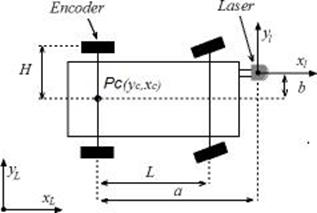
\includegraphics[width=0.6\linewidth]{image008.jpg}
    \caption{Vehicle kinematics}
    \label{fig:truck_kinematics_1}
\end{figure}
Furthermore, we have an observational model of the form
\begin{equation}
 \begin{bmatrix}
z_r \\ z_\beta  
\end{bmatrix}   
= h(x) = 
 \begin{bmatrix}
 \sqrt{ (x_L-x_v)^2 + (y_L-y_v)^2 } \\
 \arctan\left(\frac{y_L-y_v}{x_L-x_v}\right) - \phi + \frac{\pi}{2}
 \end{bmatrix} 
\end{equation}
where $(x_L,y_L)$ are the coordinates of a landmark.
\begin{figure}[H]
    \centering
    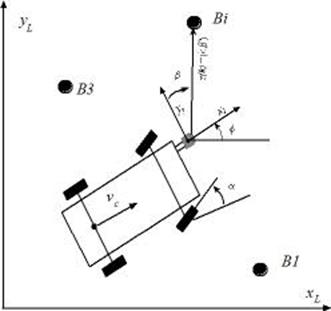
\includegraphics[width=0.5\linewidth]{image010.jpg}
    \caption{Vehicle and Laser sensor}
    \label{fig:truck_kinematics_2}
\end{figure}
\begin{enumerate}
    \item Compute the motion model Jacobian, where $(x_v,y_v,\phi_v)$ are the state variables.
    The motion model Jacobian is given by
%     \begin{align*}
%     \begin{bmatrix}
%      v_c\cos(\phi) - a \sin(\phi) -b\cos(\phi) & 0 & a\sin(\phi) -b\cos(\phi) + \Delta T\left(-v_c\sin(\phi) -\frac{v_c}{L}\tan(\alpha) (a\cos(\phi)-b\sin(\phi)) \right)
%      \\
%      0 & v_c \sin(\phi) + a \cos(\phi) - b \sin(\phi) & a\cos(\phi)-b\sin(\phi) + \Delta T \left(v_c \cos(\phi) + \frac{v_c}{L}\tan(\alpha)(-a\sin(\phi) - b \cos(\phi)) \right)
%      \\
%      0 & 0 & v_c \tan(\alpha)
%      \end{bmatrix}
%     \end{align*}
\begin{align*}
    \begin{bmatrix}
     1 & 0 & \Delta T\left(-v_c\sin(\phi) -\frac{v_c}{L}\tan(\alpha) (a\cos(\phi)-b\sin(\phi)) \right)
     \\
     0 & 1 & \Delta T \left(v_c \cos(\phi) + \frac{v_c}{L}\tan(\alpha)(-a\sin(\phi) - b \cos(\phi)) \right)
     \\
     0 & 0 & 1
     \end{bmatrix}
    \end{align*}

    \item Compute the measurement model Jacobian, where $(x_v,y_v,\phi_v,x_L,y_L)$ are the state variables (assume a single landmark).
    The measurement model Jacobian is
    

\end{enumerate}


    \end{enumerate} 
    \begin{align*}
     \begin{bmatrix}
      -(x_L-x_v)\left((x_L-x_v)^2 + (y_L-y_v)^2 \right)^{-1/2} & \frac{y_L-y_v}{(y_L-y_v)^2+(x_L-x_v)^2}\\\ 
      -(y_L-y_v)\left((x_L-x_v)^2 + (y_L-y_v)^2 \right)^{-1/2} & -\frac{x_L-x_v}{(y_L-y_v)^2+(x_L-x_v)^2}\\ 
      0 & -1\\ 
      (x_L-x_v)\left((x_L-x_v)^2 + (y_L-y_v)^2 \right)^{-1/2} & -\frac{y_L-y_v}{(y_L-y_v)^2+(x_L-x_v)^2} \\ 
      (y_L-y_v)\left((x_L-x_v)^2 + (y_L-y_v)^2 \right)^{-1/2} & \frac{x_L-x_v}{(y_L-y_v)^2+(x_L-x_v)^2}
      \\
      %
     \end{bmatrix}^T
    \end{align*}


\section{Part 2 - EKF SLAM (70 Points)}

In this problem we will be implementing a full SLAM system based on an extended Kalman filter.
The data we will be using was taken from a pickup truck equipped with a wheel encoder, GPS, and LIDAR scanner. 
The dataset we are using consists of this truck making several loops around a park with trees. 
See~\ref{fig:vic_truck} for a picture of the data collection vehicle and the environment.
\begin{figure}
    \centering
    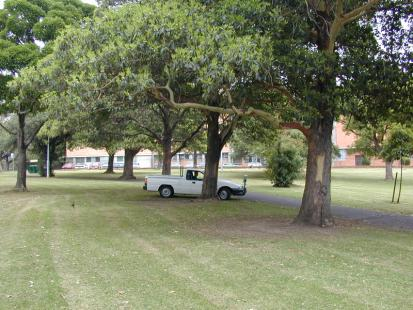
\includegraphics[width=0.8\linewidth]{truck.jpg}
    \caption{SLAM data collection vehicle}
    \label{fig:vic_truck}
\end{figure}
The vehicle model is the same as in question 1.3 above; the specific parameters corresponding to the vehicle dimensions and sensor placement are provided in the code.

Our map will consist of the centers of the trees in the park as point features in 2D, and our vehicle state will be the usual 2D vehicle state $[x\ y\ \phi]$.
To incorporate the map itself within our estimation, we need to include them as well within our EKF's state vector.
Thus, for a map that currently includes $n$ tree landmarks, the full state vector $\mat{x}$ will be given as the $3+2n$ dimensional vector
\begin{align}
    \mat{x}= \bmat{x & y & \phi & \mat{f}_1^T & \dots & \mat{f}_n^T}^T
\end{align}
where $\mat{f}_i = [x \ y]^T$ is the 2D position estimate of the $i$th tree center feature. 

From each laser scan, we begin by extracting tree features from the environment by detecting appropriately shaped clusters of laser measurements, estimating the trunk diameter, and finally estimating the range and bearing to the trunk center from the truck's position.
This has already been implemented for you as \texttt{extract\_trees} within the \texttt{tree\_extraction} package.

Note that as these real measurements aren't time synchronized perfectly or even coming in at the same frequency, we won't have simple propagate-update iterations, but rather must process odometry/GPS/laser events as they become available to us.
High level pseudocode of the entire SLAM algorithm can be written as in Algorithm~\ref{alg:slam}.
\begin{algorithm}[t]
{\small%\footnotesize
  \begin{algorithmic}[1]
    \While{filter running}
    \State $e \leftarrow$ next event to process
    \If{$e$ is an odometry event}
      \State Perform EKF propagation with $e$
    \ElsIf{$e$ is a GPS measurement}
      \State Perform an EKF update with $e$
    \ElsIf{$e$ is a laser scan}
      \State Extract tree range, bearing measurements $\{z\}$ from $e$
      \State Perform an EKF update with $\{z\}$
    \EndIf
    \EndWhile
  \end{algorithmic}
}
\caption{: EKF SLAM}
\label{alg:slam}
\end{algorithm}

After extracting a measurement $\mat{z}_j = (r, b)$ of a tree trunk in the environment from a laser scan, we do not know a priori \emph{which} tree in our state vector this tree corresponds to.
The measurement Jacobians and hence EKF update will take a different form depending on whether measurement $\mat{z}_j$ is an observation of $\mat{f}_1$ or $\mat{f}_6$, so before we perform the EKF update we must first decide which measurements $j$ correspond to which landmarks $i$.
Furthermore, there is the possibility that the measurement corresponds to a tree that currently is not even in our map, requiring us to initialize a new landmark and expand our state vector.
This is known as the problem of \emph{data association}.

We have included several plotting utilities that should aid your development. 
They are contained in the \texttt{slam\_utils} package and should run by simply calling \texttt{init\_plot} and then \texttt{do\_plot} with your current \texttt{ekf\_state}.
Laser measurements are displayed \emph{green} if they are associated with an existing mapped landmark, \emph{blue} if they correspond to initialization of a new landmark, or \emph{red} if they were thrown out and not used. 
The plotting code requires \texttt{PyQt5} and \texttt{pyqtgraph}; \texttt{matplotlib} has a simpler interface but is too slow for real-time visualization as done here.
The plot will auto-scale as the map expands, or you can manually zoom in and pan with the mouse.
Plotting the covariance ellipse for every estimated landmark is useful but takes a significant amount of time; this can be disabled by setting \texttt{filter\_params["plot\_map\_covariances"] = False}.


\subsection{Odometry Propagation}
We will begin by implementing the propagation steps of the EKF.
The motion model and Jacobians were given or derived in question 1.3 above.
On completing both subsections below, you should be able to run the code and see a moving (though very inaccurate) estimate of the truck's position, along with a quickly growing $3\sigma$ covariance ellipse.

\subsubsection{Vehicle motion model}
Implement the vehicle motion model and its Jacobian in the function \texttt{motion\_model}

\subsubsection{EKF Propagation}
Implement the EKF odometry propagation in the function \texttt{odom\_predict}

\subsection{GPS Update}
Implement the GPS update equations in the function \texttt{gps\_update}.
GPS measures position directly, so the measurement equation is simply $h(\mat{x}) = [ x \ y ]^T$.
After completing this, you should have a much improved filter; on each GPS measurement, the estimate should jump back towards the true value and the covariance ellipse should shrink significantly.

Due to the nature of GPS there are a few measurements within the given data that are erroneous and should be thrown out.
In an EKF update, the innovation or residual $\mat{r}$ and residual covariance $\mat{S}$ are useful for determining if a measurement is consistent with your current state estimate.
Let the \emph{Mahalanobis distance} of this residual be given as the scalar quantity
\begin{align}
    d(\mat{r}, \mat{S}) = r^T \mat{S}^{-1} r
\end{align}

Because the residual is normally distributed with covariance $\mat{S}$, $d$ follows a known distribution, a $\chi^2$ distribution with $m$ degrees of freedom, where $m$ is the dimension of $\mat{r}$ (2 in this case).
Thus, we can use this known distribution to exclude measurements that are extremely unlikely given our model and estimate.
Excluding measurements with probability less than 0.001 corresponds to throwing out any measurements with $d(\mat{r}, \mat{S}) > \texttt{chi2inv}(0.999, 2)$ where \texttt{chi2inv}(.999,2) is the inverse of the $\chi^2(2)$ cdf at $p = 0.999$, or about 13.8.



\subsection{LIDAR update}

Finally we will complete the implementation by incorporating the laser measurements.
The measurement model and Jacobians were given or derived in question 1.3 above.

\subsubsection{Range and bearing measurement model}
Implement the range and bearing measurement model given above, as well as its Jacobian that you derived, in the function \texttt{laser\_measurement\_model}.

\subsubsection{Landmark initialization}
Implement the function \texttt{initialize\_landmark} that initializes a new landmark in the state vector from a measurement $\mat{z}$.
You'll need to use the inverse of the measurement function, $h^{-1}(\mat{z})$, and don't forget you also need to expand the covariance matrix $\mat{P}$ to match the newly expanded $\mat{x}$.

\subsubsection{Data association}
Implement the function \texttt{compute\_data\_association} that computes the measurement data association as discussed above.
Given an input state $(\mat{x}, \mat{P})$ and set of measurements $\{z\}$, the function should return an array \texttt{assoc} such that \texttt{assoc[j] == i} if measurement $j$ was determined to be associated with landmark $i$.
Furthermore there are two special cases: if \texttt{assoc[j] == -1}, measurement $j$ was determined to be an observation of a new landmark requiring initialization; if \texttt{assoc[j] == -2}, measurement $j$ was determined to be too ambiguous to use and should be completely thrown out.

For given measurements $\mat{z}_k$ and landmarks $\mat{f}_j$, the Mahalanobis distance between $\mat{z}_k$ and the expected measurement of $\mat{f}_j$, $h(\mat{x}, \mat{f}_j)$, is a useful metric to determine how likely it is that the measurement is an observation of that feature.
The residual covariance $\mat{S}$ that you will use in this calculation is computed the same as it is in the EKF update step, and the Mahalanobis distance then has the same form $d = \mat{r}^T \mat{S}^{-1} \mat{r}$. 
Recall from the above discussion of this metric that $d$ follows a known $\chi^2$ distribution.

You may find the function \texttt{slam\_utils.solve\_cost\_matrix\_heuristic} useful here. 
Given a matrix of costs $\mat{M}$, where $m_{ij}$ is thought of as the cost of assigning some entity $i$ to some entity $j$, this function attempts to find a minimum total cost matching such that each $i$ is assigned to some $j$.
It returns a list of matching pairs $(i,j)$.
This function is heuristic and suboptimal but runs efficiently and should be good enough for this use case; the optimal method known as the Hungarian or Munkres algorithm can be used instead.

You will probably need to disregard ambiguous measurements, both in the sense of those that could be matched to two known landmarks with similar cost, and in the sense of those that are on the border between being matched to a known landmark and being initialized as a new landmark.
The known distribution of $d$ will be useful here.

\subsubsection{Laser update}
Finally, implement the EKF update from tree detections in the function \texttt{laser\_update}.
After implementing the laser updates, it's important that you verify that the filter functions correctly with or without GPS updates enabled.

\subsection{Miscellaneous advice}

\begin{enumerate}

\item Any time you modify the covariance matrix $\mat{P}$, numerical issues may cause it to become slightly non-symmetric.
It is thus useful to assign $\mat{P} \leftarrow \frac{1}{2}(\mat{P} + \mat{P}^T)$ after each such update, or call the function \texttt{slam\_utils.make\_symmetric}.

\item Similar to the above, small numerical issues may cause the eigenvalues of $\mat{P}$ to become slightly negative over time.
If you observe this happening (and only if), it may be remedied by adding a small constant times the identity to $\mat{P}$ to increase its eigenvalues by the same amount: $\mat{P} \leftarrow \mat{P} + \kappa \mat{I}$ for small $\kappa$.
See the function \texttt{slam\_utils.plot\_covariance} where we set $\mat{P} \leftarrow \mat{P} + \left(\lambda_{min}(\mat{P}) + 10^{-6}\right) \mat{I}$ if necessary in order to take the Cholesky decomposition.

\item Due to the periodic nature of SO(2) and the angle $\phi$, it is important to project the angle back into the range $[-\pi, \pi)$ after each operation.
The function \texttt{slam\_utils.clamp\_angle} can do this for you.

\end{enumerate}

\end{document}
